% evaluation_pipeline_v1.tex — FIGURE SCAFFOLD, NOT PROSE.
%
% Places the five final timing figures under the research objectives named in the threat
% model (RO1 read timing, RO2 control timing, RO3 safety), so every figure is referenced from
% the manuscript and the evaluation is organised 1:1 against the objectives as the structure
% contract requires. The section body is empty on purpose: the evaluation text has not been
% written and must be drafted through the pipeline (draft -> paper-voice -> academic-humanizer
% -> lin_check) before submission.
%
% Figures live in figures/timing/ and are included at NATURAL size (no width= scaling): the
% PDFs are produced at IEEE column measure, 8.5 pt Times, by defense4/timing/reproduce.sh.
% Provenance for every figure: ../FIGURE_PROVENANCE.md and ../FINAL_FIGURES.md.
%
% Claim boundaries every sentence written here must respect (CLAIMS_AND_LIMITATIONS.md in
% defense4/timing/):
%   * Both arms ran the same unified switch binary with the size-shaping datapath active; the
%     Timing OFF arm is NOT an unmodified native SEL-751 baseline. The comparison isolates the
%     timing-mode change within one binary.
%   * SELECT means the SELECT phase of SBO (function 3), not a complete SBO transaction.
%   * Figures 1-3 and 5 are READ-versus-SELECT transaction timing, not device identification.
%   * Figure 4 reports only master-visible OPERATE timing. J was NOT observed on the
%     relay-facing wire; exactly-once relay delivery is NOT demonstrated.
%   * Configuration provenance is PARTIAL (one archived readback reports an unrecoverable
%     failed assertion).
%   * The Timing ON mutual-information estimate is quoted as "below 0.003 bits and inside the
%     permutation null", not to four significant figures.

\section{Evaluation}
\label{sec:eval}

% TODO: testbed and method paragraph. One Tofino-1 between the master and one physical
% SEL-751; six master-facing captures, one session, 2026-08-13; arms = Timing OFF / Timing ON.

\subsection{Effectiveness in RO1 (read timing)}
\label{sec:eval:ro1}

% TODO: prose for RO1.

\begin{figure*}[t]
  \centering
  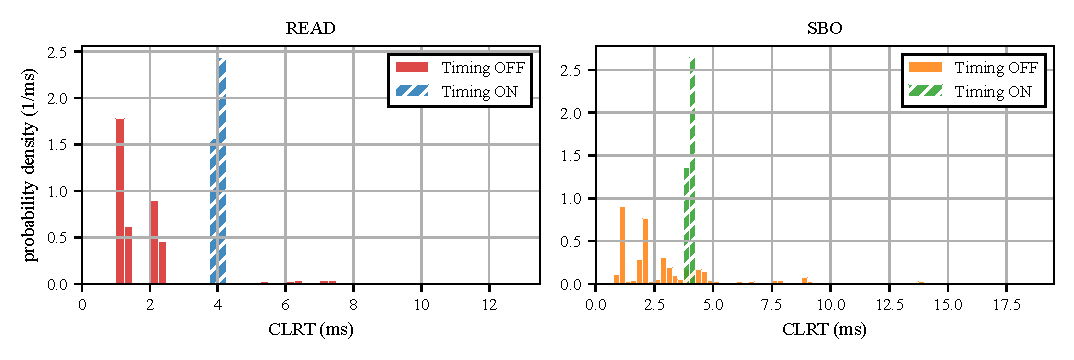
\includegraphics{figures/timing/fig01_clrt_read_select_before_after}
  \caption{Cross-layer response time (CLRT), the interval from the outstation's TCP
    acknowledgment to its DNP3 application response, with the timing mechanism disabled
    (Timing OFF) and enabled (Timing ON), measured master-facing against the physical SEL-751.
    Left: READ (function~1). Right: the SELECT phase of select-before-operate (function~3);
    these are SELECT observations, not complete SBO transactions. With the timing mode off,
    CLRT is spread over roughly 1 to 18~ms and differs between the two transaction types; with
    it on, both collapse onto a 4.001~ms policy value (dashed line) with a standard deviation
    of about 0.02~ms. Each panel's horizontal axis runs to its largest observation, so the full
    tail is visible. Both arms ran the same unified switch binary with the size-shaping
    datapath active; the Timing OFF arm is therefore not an unmodified device baseline, and
    the comparison isolates the timing-mode change.}
  \label{fig:clrt-dist}
\end{figure*}

\begin{figure}[t]
  \centering
  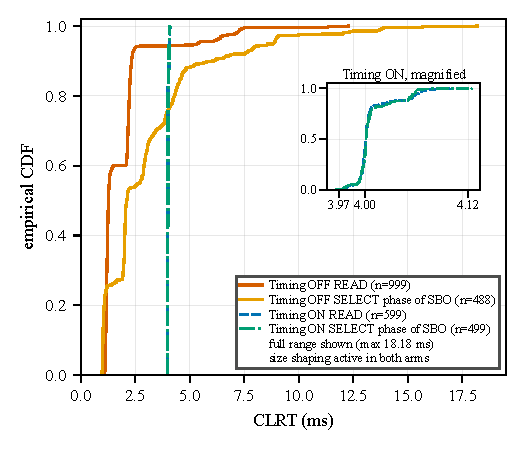
\includegraphics{figures/timing/fig02_clrt_ecdf_before_after}
  \caption{Empirical CDF of CLRT for READ and for the SELECT phase of SBO with the timing
    mechanism disabled (solid) and enabled (dashed). With the timing mode off the two
    transaction types separate clearly and the SELECT distribution carries a tail to
    18.18~ms, shown in full; with it on, both collapse onto 4.001~ms, and the inset resolves
    the two Timing ON curves, which coincide at full scale. Size shaping was active in both
    arms.}
  \label{fig:clrt-ecdf}
\end{figure}

\begin{figure*}[t]
  \centering
  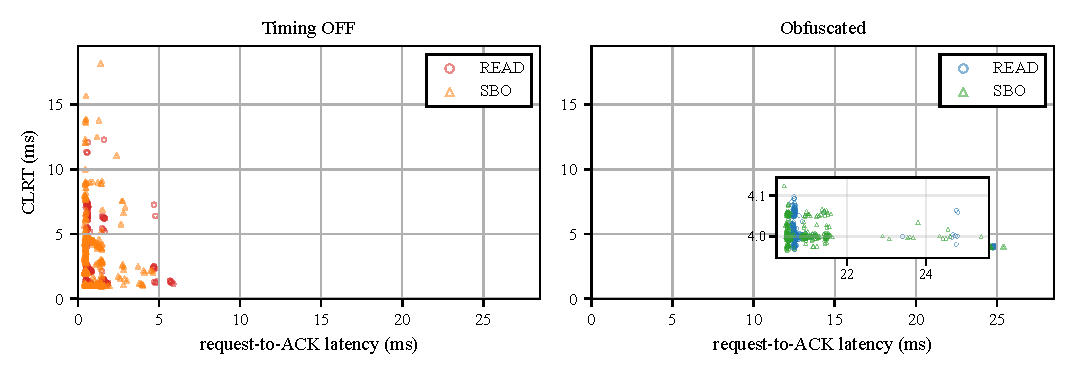
\includegraphics{figures/timing/fig03_timing_feature_overlap_before_after}
  \caption{Timing-feature overlap with the timing mechanism disabled and enabled. Each point
    is one transaction, placed by the two latencies a passive observer can measure
    master-facing: request-to-ACK on the horizontal axis and ACK-to-response (CLRT) on the
    vertical. Left, timing mode off: READ and the SELECT phase of SBO occupy visibly different
    regions. Right, timing mode on: both transaction types collapse onto a single point and
    are no longer separable by these features. This is a display of feature overlap between
    two transaction types on one relay, not a clustering result and not device
    identification; no unsupervised algorithm is fitted.}
  \label{fig:overlap}
\end{figure*}

\begin{figure*}[t]
  \centering
  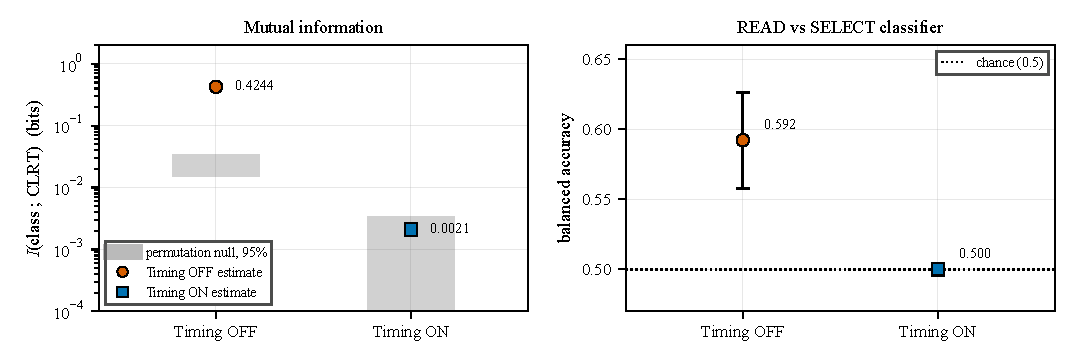
\includegraphics{figures/timing/fig05_timing_leakage_summary}
  \caption{Timing-only leakage with the timing mechanism disabled and enabled. Left: mutual
    information between transaction class and CLRT, with the shaded band giving the 95\,\%
    permutation null for each arm; with the timing mode off, CLRT carries about 0.42~bits
    about whether a transaction was a READ or the SELECT phase of an SBO, and with it on the
    estimate falls inside its own null band. Right: balanced accuracy of a classifier trained
    on Timing OFF CLRT to separate the two transaction types, applied unchanged to Timing ON
    traffic, falling from 0.592 to chance. Both panels describe transaction-class feature
    suppression on a single SEL-751 in a single capture session with a transaction-disjoint,
    not session-disjoint, split; neither is a device-identification result.}
  \label{fig:leakage}
\end{figure*}

\subsection{Effectiveness in RO2 (control timing)}
\label{sec:eval:ro2}

% TODO: prose for RO2. Valid statement: the master-visible echo-minus-ACK interval remained
% approximately 4.00 ms across the configured J values of 2, 6 and 12 ms. J is the configured
% codebook value; it was not observed on the relay-facing wire.

\begin{figure*}[t]
  \centering
  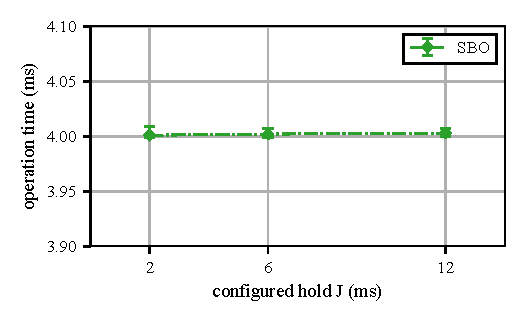
\includegraphics{figures/timing/fig04_sbo_operate_timing_by_j}
  \caption{OPERATE timing under three configured hold values. Left: the master-visible
    request-to-ACK delay $A$ and request-to-echo delay $R$, both flat in $J$. Right: the
    echo-to-ACK interval $R-A$, which stays at about 4.00~ms across $J = 2$, 6 and 12~ms, so
    an observer who subtracts the two observable timestamps learns nothing about the
    configured hold. Markers are medians of 30 OPERATE transactions per condition; bars are
    bootstrap 95\,\% confidence intervals on the median. $J$ is the configured codebook
    value; it was not observed on the relay-facing wire, and exactly-once relay delivery is
    not demonstrated.}
  \label{fig:operate-j}
\end{figure*}

\subsection{Safety in RO3}
\label{sec:eval:ro3}

% TODO: prose for RO3. Evidence: defense4/timing/evidence/final_read_sbo/readbacks/
% relay_outputs_final.json (all relay outputs open before, during and after every batch;
% guarded points {1,3} only; index 6 refused).
